\section{Panoramica dello Stato dell'Arte}

\subsection{Epidemiologia}
L'epidemiologia rappresenta una disciplina biomedica di fondamentale 
importanza, focalizzata sull'analisi della distribuzione e dell'incidenza 
delle malattie e degli eventi sanitari rilevanti all'interno di una 
popolazione. Questo campo di studio si dedica all'approfondimento 
delle cause, dei pattern temporali e delle conseguenze delle malattie 
\cite{Galea2009-lj} \cite{Parascandola2001-kw}.

L’epidemiologia si divide in quattro ambiti principali \cite{rothman2015modern}: epidemiologia
descrittiva, epidemiologia analitica, epidemiologia clinica ed epidemiologia
sperimentale.

\begin{enumerate}
    \item \textbf{L’epidemiologia descrittiva} si occupa di studiare la
    frequenza e la distribuzione delle malattie e dei parametri di salute
    nelle popolazioni. Descrive eventi sanitari come malattie, cause di morte 
    la presenza di fattori di rischio come, ad esempio, il fumo di tabacco,
    l’inquinamento atmosferico.
    \item \textbf{L’epidemiologia analitica} si occupa invece di studiare le
    cause delle malattie e degli eventi sanitari. In particolare, cerca di 
    identificare i fattori che possono influenzare l’insorgenza o lo sviluppo
    della malattia.
    \item \textbf{L’epidemiologia clinica} si concentra sullo studio dei
    pazienti affetti da una determinata patologia. In particolare, cerca di
    identificare i fattori che possono influenzare il decorso della malattia
    e l’efficacia dei trattamenti.
    \item \textbf{L’epidemiologia sperimentale} si occupa invece di studiare 
    gli effetti delle terapie preventive o curative sulla popolazione.
\end{enumerate}

L'epidemiologia si caratterizza per la sua natura essenzialmente 
pratica, poiché il suo obiettivo principale consiste nel determinare 
le cause sottese a un determinato effetto sanitario. Questa disciplina 
si trova ad affrontare una serie di sfide complesse che definiscono 
il suo percorso. Tra queste sfide possiamo trovare l'identificazione 
delle relazioni di causalità tra eventi.

Tali interrogativi possono sembrare elementari, dato che, come specie, 
abbiamo sviluppato un istinto innato nell'individuare correlazioni 
causali tra eventi, anche quando queste non esistono effettivamente. 
Ad esempio, se ci trovassimo in un bosco buio, soli e circondati 
solo dal sussurro di una leggera brezza estiva e dovessimo udire un 
rumore provenire dai cespugli, è probabile che lo assoceremmo a un 
pericolo imminente, come la presenza di un predatore, sebbene il 
rumore sia causato dalla brezza stessa.

Questo adattamento evolutivo ci ha permesso di sopravvivere in 
situazioni di pericolo, ma purtroppo, quando si tratta di scienza e dati, 
l'istinto non è sempre una guida affidabile. I dati, per loro natura, 
sono neutri e non trasmettono automaticamente informazioni significative; 
spetta a noi, in quanto individui dotati di intelligenza, 
tecniche e metodi, estrarre significato da questi dati in modo accurato 
ed inequivocabile.

Un'osservazione chiave è che ciò che sembra ovvio può essere fuorviante. 
Per esempio, il grafico seguente sembra dimostrare in modo 
``inequivocabile'' una relazione diretta tra la spesa degli Stati Uniti 
per la ricerca aerospaziale e il numero di suicidi per strangolamento:

\begin{figure}[H]
    \begin{center}
        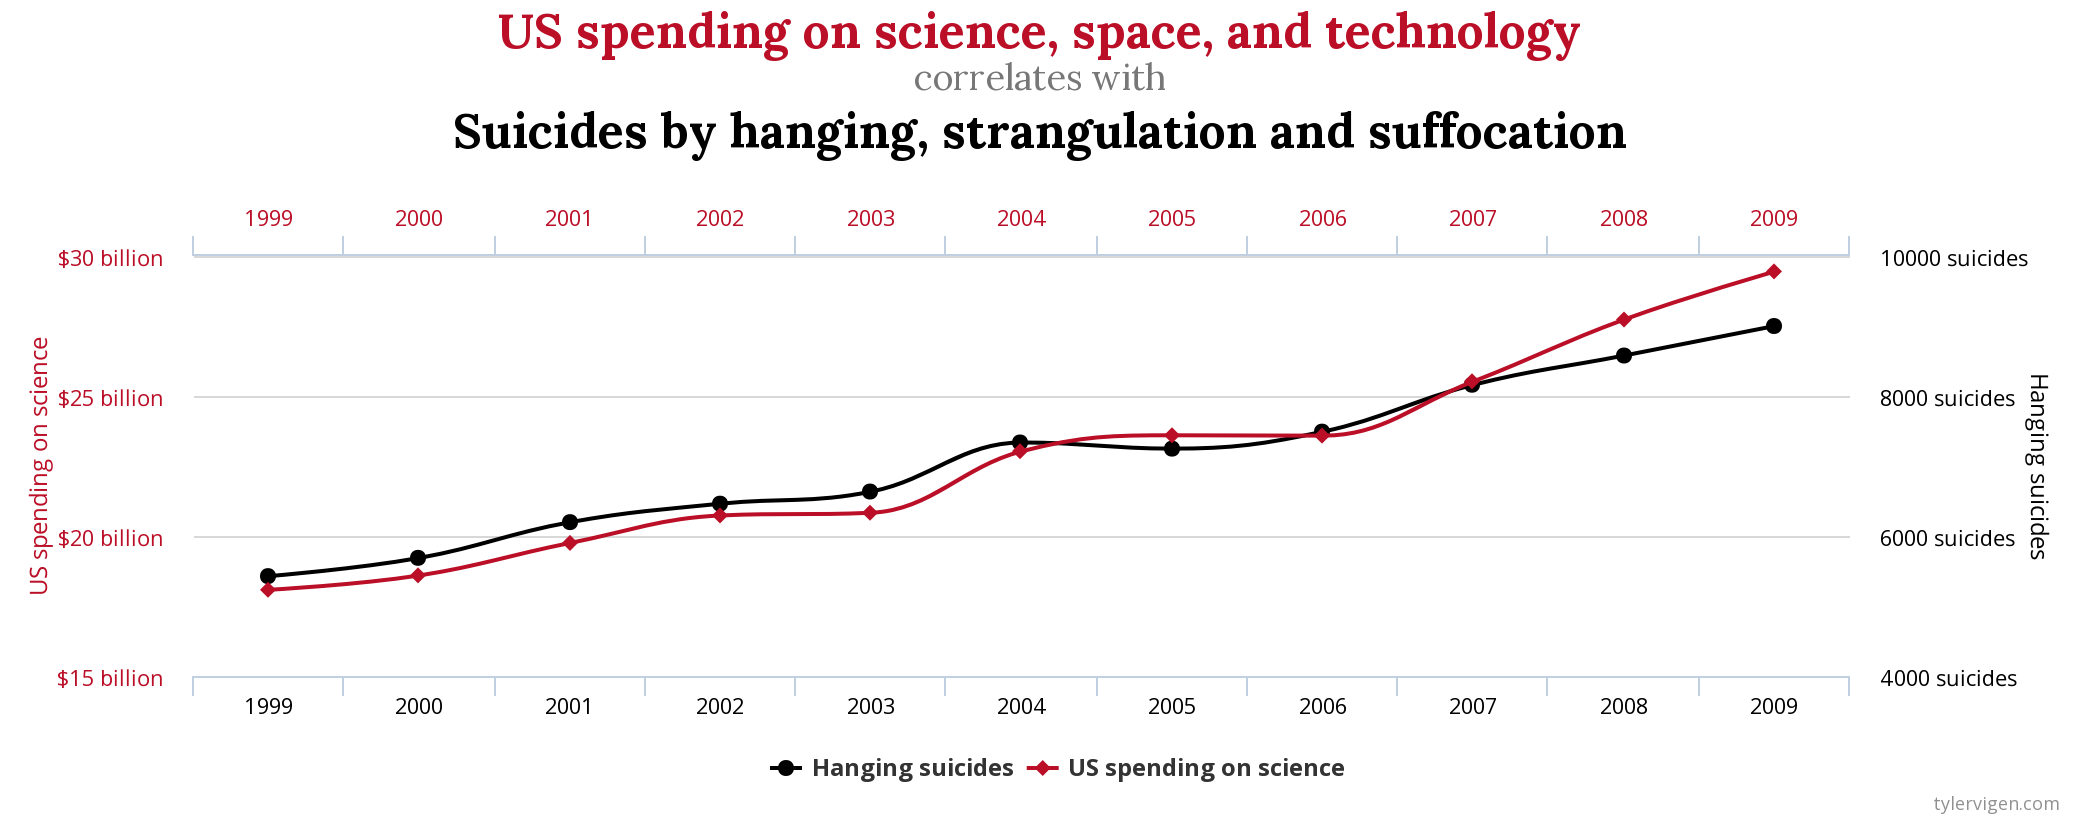
\includegraphics[width=\linewidth]{img/chart.png}
        \caption{Esempio di correlazione spuria}
        \url{https://www.tylervigen.com/spurious-correlations}
        \label{fig:spurious_relations}
    \end{center}
\end{figure}

Sulla base di questo grafico e dei dati presentati, si potrebbe 
erroneamente concludere che le due categorie sono in qualche modo 
correlate e che il governo degli Stati Uniti debba essere 
accusato di incitare al suicidio. Tuttavia, questo è un esempio 
di una relazione spuria, in cui due o più variabili sono 
associate ma non sono causalmente collegate.

È importante sottolineare che l'associazione e la causalità non sono 
la stessa cosa, e quando si studia una, è fondamentale non confonderla 
con l'altra. In statistica, una correlazione tra dati rappresenta 
qualsiasi tipo di relazione tra due o più variabili, indipendentemente 
dalla sua natura causale o non causale. Nel caso precedente, 
la correlazione tra le due variabili potrebbe essere semplicemente 
dovuta al passare del tempo: nel corso degli anni, la spesa media per 
la ricerca aerospaziale è continuata a crescere a causa di un interesse 
e di investimenti sempre maggiori in quel settore, mentre nel tempo 
si è verificato un costante aumento del numero di suicidi.

Il nostro pregiudizio verso la ricerca di collegamenti tra eventi, 
in modo che sembrino sempre collegati in modo tangibile e che si 
possa tracciare una chiara e distinta linea causale dall'inizio alla 
fine, può ingannarci quando tali collegamenti sembrano evidenti ma 
non lo sono. Spesso, la spiegazione più semplice è anche la meno 
interessante, sebbene sia corretta: due eventi completamente svincolati 
tra loro possono avere andamenti simili, e differenti fattori possono 
portare allo stesso comportamento. 

Il problema della causalità è di estrema importanza e rappresenta 
una delle sfide principali quando si cercano di sviluppare e 
applicare interventi all'interno di una popolazione per mitigare, 
ad esempio, la diffusione di un agente patogeno \cite{Parascandola2001-kw}.

Come già accennato, i dati per se stessi sono privi di significato; 
è il nostro compito imparare a interpretare il loro significato. 
Un esempio eloquente di come, nonostante la consapevolezza del problema 
delle correlazioni spurie, i dati possano comunque trarre in inganno 
è il seguente:

Supponiamo di essere medici e di dover decidere se prescrivere un 
certo farmaco a un paziente. Per prendere questa decisione, abbiamo 
a disposizione la storia clinica del paziente e i risultati di uno 
studio su un nuovo farmaco che sembra promettente nel trattamento 
della sua malattia. Questo farmaco è stato testato su un gruppo di 
700 persone, suddivise in due sottogruppi di 350 pazienti ciascuno. 
I pazienti hanno scelto autonomamente se assumere o meno il farmaco.
Ecco i risultati:

\begin{table}[H]
    \centering
    \caption{Paradosso di Simpson}
    \begin{tabular}{ |p{2.2cm}||p{1.6cm}|p{1.6cm}|p{1.6cm}||p{1.6cm}|p{1.6cm}|p{1.6cm}| }
        \hline
        \multicolumn{7}{|c|}{Paradosso di Simpson} \\
        \hline
        Categoria & Pazienti & Guariti & \% Guariti & Pazienti & Guariti & \% Guariti\\
        \hline
        Uomini & 87 & 81 & 93\% & 270 & 234 & 87\% \\
        Donne & 263 & 192 & 73\% & 80 & 55 & 69\% \\
        Dati combinati & 350 & 273 & 78\% & 350 & 289 & 83\% \\
        \hline
    \end{tabular}
\end{table}

Questi risultati sembrano suggerire che la prescrizione di questo 
nuovo farmaco non abbia un impatto positivo sulla guarigione dei 
pazienti. Tuttavia, questo risultato è in realtà un esempio del 
cosiddetto ``paradosso di Simpson'', in cui i dati aggregati relativi 
a un trattamento specifico sembrano indicare una perdita di efficacia, 
mentre i dati delle singole categorie mostrano risultati opposti. 
Questo esempio sottolinea il fatto che l'interpretazione di dati 
aggregati non sempre può essere affidabile, e talvolta può ingannare. 
In questi casi, è necessario estrarre le informazioni sulla causalità 
dai dati individuali.

È evidente che comprendere le cause di un determinato effetto o 
insieme di effetti non è un compito banale. Anche conoscendo 
l'agente patogeno o almeno la sua natura, non sempre è sufficiente 
per spiegare la complessità delle interazioni. 
L'utilizzo di modelli di apprendimento automatico per l'analisi dei 
dati, la ricerca di correlazioni e la successiva formulazione di 
politiche di intervento può rappresentare un rischio, ma al contempo 
offre un alleato potente nella definizione di politiche di intervento 
in settori estremamente delicati come quello della sanità 
\cite{doi:10.1098/rsos.220638}.